\section{Medidor de Correlación}
El medidor de correlación monitoriza la salida stereo de Traverso y muestra el coeficiente de correlación entre los canales izquierdo y derecho. A diferencia de otros medidores de correlación, éste interpreta el coeficiente como una medida de la amplitud del stereo, y dibuja un gradiente que representa el campo stereo.

Para explicar qué es la correlación y porqué es importante, pensemos que una onda senoidal pura se reproduce por los canales izquierdo y derecho del master. Cuando ambas señales se mezclan (lo que ocurre en una reproducción mono), la señal resultante es la suma de los canales izquierdo y derecho. Dependiendo de la diferencia de fase entre las señales originales, se obtienen distintos efectos de interferencia: si en un instante las amplitudes a sumar son positivas, se obtiene una amplitud resultante mayor, mientras que si una es positiva y otra negativa, la amplitud resultante será menor. En casos especiales (``oposición de fase''), se suma un valor positivo con uno negativo similar en todos los instantes, y puede llegarse a no obtener más que silencio (\FigB\ \ref{fig_interference}).

\begin{figure}
	\centering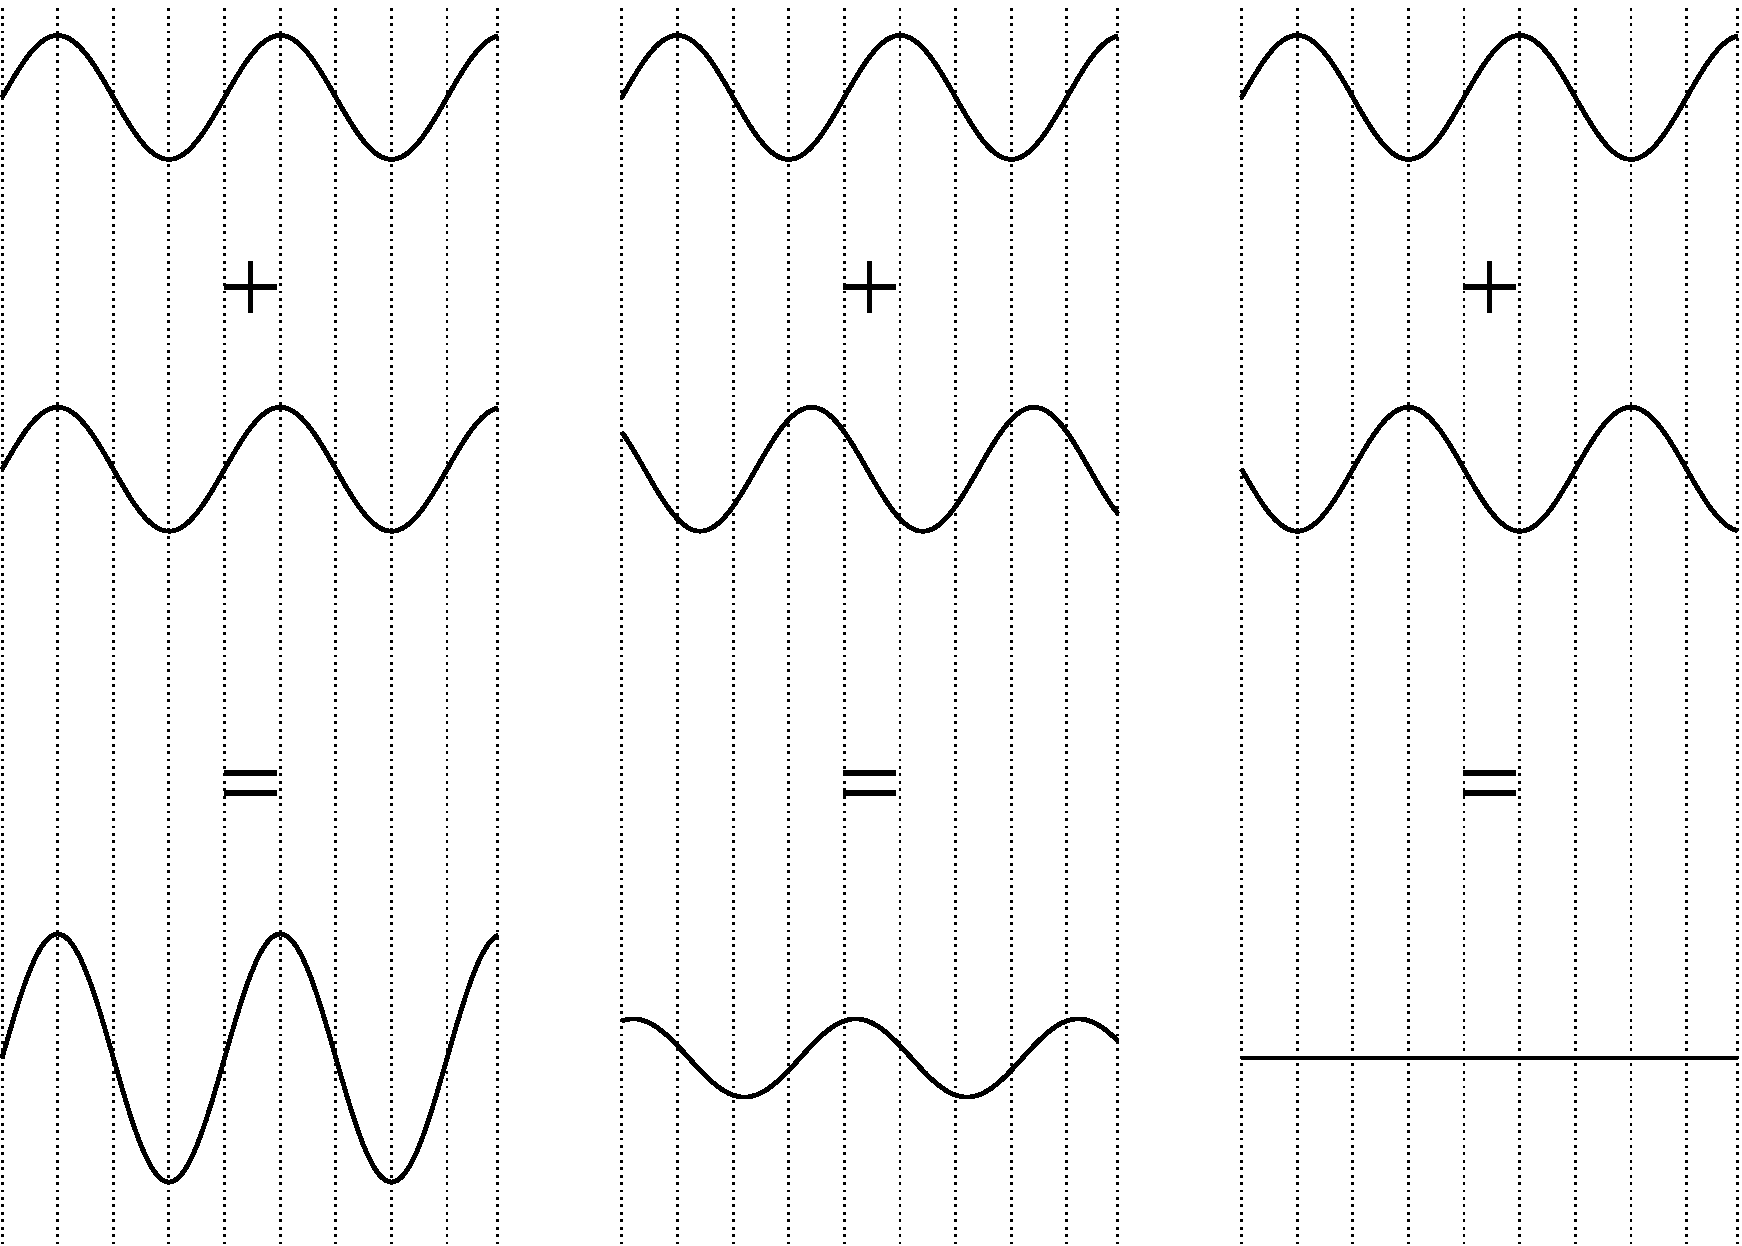
\includegraphics[width=0.5\textwidth]{../images/sine01}
	\caption{Cuando se suman dos ondas senoidales, la interferencia puede producir una amplificación (ondas en fase, a la izda.), una onda de aproximadamente la misma amplitud (sin correlación, al centro), o una amplitud nula (oposición de fase, a la dcha.).}
	\label{fig_interference}
\end{figure}

Si las dos señales originales contienen datos más complejos, por ej. música o voz hablada, los efectos de cancelación (conocidos como \emph{cancelaciones de fase}), no cancelan completamente la señal, sino que sólo atenúan algunas frecuencias, produciendo un sonido ``hueco'' y en general extraño. No hay que insistir en que estos efectos son nefastos para una producción de audio de calidad. Aunque es indiscutible que debemos usar nuestros oídos y escuchar la señal en mono para detectar problemas de fase, los programas de audio digital proporcionan ayudas visuales de varios tipos para analizar la señal de audio. Esta es una de las razones por la que muchos usuarios prefieren usar estaciones digitales de audio. Hay varias maneras de representar la correlación visualmente, pero para entender cómo se interpreta el medidor de correlación de Traverso, es necesaria alguna explicación más.

La cantidad de correlación se representa por el valor del \emph{coeficiente de correlación lineal} $r$, que se se calcula a partir de una matriz que contiene pares de muestras $(x_i,y_i)$:
\[
r = \frac{\sum\limits_{i}(x_i - \bar{x})(y_i - \bar{y})}{\sqrt{\sum\limits_{i}(x_i - \bar{x})^2} \sqrt{\sum\limits_{i}(y_i - \bar{y})^2}}
\]

$r$ está entre $-1.0$ y $1.0$. Un valor de $r = 1.0$ significa que el canal derecho e izquierdo están perfectamente correlacionados. La señal original sería mono en este caso, ya que no hay diferencia de fase entre los canales. Cuanta más diferencia haya entre los canales, menor será el coeficiente de correlación. En caso de datos sin ninguna correlación (lo que podría entenderse como ``no hay similitud de fase apreciable entre el canal izdo. y el dcho.''), $r$ será 0.0. Una señal de este tipo produce una imagen stereo amplia con poco riesgo de cancelaciones de fase al sumarse en mono. La diferencia entre señales puede ser aún mayor, cuando un canal es el inverso del otro. En ese caso $r$ vale $-1.0$. Valores negativos de $r$ indican alto riesgo de cancelaciones de fase.

El medidor de correlación de Traverso (menu ``Ver $\rightarrow$ Medidor de correlación'') muestra el coeficiente de correlación de una manera intuitiva. En lugar de centrarse en el valor numérico, muestra su significado en términos de amplitud stereo (\FigB\ \ref{fig_cmeter01}). Un gradiente que prácticamente llene el espacio entre el altavoz izquierdo y el derecho (marcados por las líneas L y R), indica una señal no correlacionada ($r = 0.0$), y por tanto una imagen stereo muy amplia. Mientras el gradiente no sobrepase las líneas L y R, hay correlación positiva y por lo tanto poco riesgo de cancelaciones de fase. Pero si se extiende \emph{más allá} de esas líneas, es probable que existan cancelaciones de fase cuando la señal se sume a mono. La imagen stereo sonará antinaturalmente amplia. Esto debe evitarse a toda costa. Por otra parte, una señal mono de entrada hará que el gradiente se concentre en una sola linea en el centro.

\begin{figure}
	\centering
	\subfigure[Estereo, $r = 0.0$]{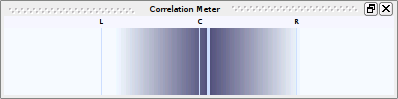
\includegraphics[width=0.5\textwidth]{../images/cmeter1}}
	\subfigure[Mono, $r = 1.0$]{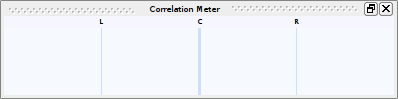
\includegraphics[width=0.5\textwidth]{../images/cmeter2}}
	\subfigure[Cancelación de fase, $r = -1.0$]{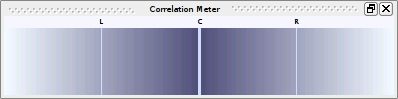
\includegraphics[width=0.5\textwidth]{../images/cmeter4}}
	\caption{El medidor de correlación de Traverso muestra el coeficiente de correlación de la señal se salida como un gradiente entre dos líneas que representan los altavoces izquierdo y derecho. Si el gradiente llena la zona entre L y R, la señal no está correlacionada (coef. de correlación $r = 0.0$), y el campo stereo es amplio (arriba). Si el gradiente se concentra en una sola línea, la señal está totalmente correlacionada ($r = 1.0$), lo que significa que la señal es mono (centro). Si el gradiente se extiende más allá de las líneas L y R, la correlación es negativa, y habrá riesgo de cancelaciones de fase audibles si la señal se escucha en mono (abajo).}
	\label{fig_cmeter01}
\end{figure}

El medidor de correlación puede usarse también para equilibrar la salida del master. Si los niveles de los canales izquierdo y derecho están bien equilibrados, la línea central del gradiente debiera ``bailar'' alrededor de la posición central.

Como el gradiente usualmente ocupa sólo el área entre las líneas L y R, el espacio exterior a esas líneas puede quedar desperdiciado casi siempre. Por eso la escala del medidor de correlación puede cambiarse pulsando \sact{M}.

\section{Analizador de espectro FFT}
Las estaciones de audio digitales suelen incorporar un analizador de espectros basado en la Transformada Rápida de Fourier (FFT). El analizador de espectros de Traverso se abre desde el menú ``Ver $\rightarrow$ Espectro FFT''. Es una ventana acoplable que puede también moverse libremente arrastrándola con el ratón.

El analizador de espectros FFT muestra la salida stereo y descompone la señal en bandas de frecuencia. Cada banda muestra el mayor valor $dB_{izdo.} + dB_{dcho.}$ en su rango (\FigB\ \ref{fig_fft1}). Puede abrirse una ventana de configuración pulsando \sact{E}, o desde el menú que aparece con \sact{Q}, o con un click del botón derecho del ratón.

\begin{figure}
	\centering
	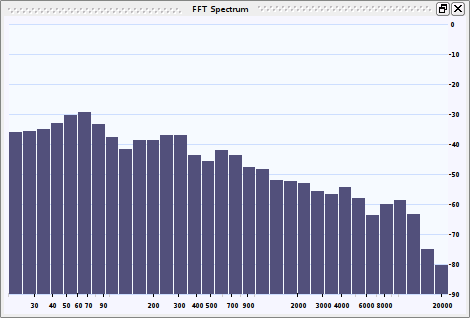
\includegraphics[width=0.5\textwidth]{../images/fft1.png}
	\caption{El  analizador de espectros FFT descompone la señal de salida del master en sus frecuencias.}
	\label{fig_fft1}
\end{figure}

La ventana de configuración mostrada en \FigT\ \ref{fig_fft3} permite definir el rango de dB y de frecuencia que se mostrará. El espectro audible va desde 20 hasta aproximadamente 18000 Hz, y la calidad CD cubre desde 20 hasta 22050 Hz. Por eso los valores recomendados para las frecuencias inferior y superior son de ese orden. El límite superior para los valores en dB del eje vertical se pone normalmente entre $-6$ y $+6$ dB, y el límite inferior entre $-60$ y $-120$ dB. El número de bandas puede elegirse a voluntad, pero números altos ($\geq 128$) pueden cargar notoriamente a la CPU.

La característica ``mostrar espectro promedio'' activa una curva que calcula el espectro promedio en el tiempo, acumulando los valores según Traverso reproduce. La curva se inicializa si se reinicia la reproducción, o mediante la acción de teclado \sact{L}. La curva promedio puede también alternarse con la normal mediante \sact{M}. Tan pronto como haya promedios disponibles, la curva puede exportarse ya sea como una lista de números o en formato \texttt{grace}, que puede ser abierto con el programa XmGrace (acción de teclado \dact{Return}).

En la sección ``Opciones avanzadas'' pueden configurarse otros parámetros relacionados con el cálculo de la FFT. El tamaño de la FFT determina el límite inferior del espectro: mayores tamaños lo extienden a frecuencias menores, a costa de más uso de CPU. La frecuencia menor que procesa el algoritmo FFT es:
\[
f_{min} = \frac{\textrm{TasaDeMuestreo}}{\textrm{Tamaño FFT}}
\]
La frecuencia \emph{más baja} en una transformada FFT de 1024 muestras de una señal de audio de muestreada a 44100~Hz resulta ser 43.1~Hz. Aumentar el tamaño de la FFT a 2048 muestras extiende el rango hasta 21.5~Hz. La \emph{mayor} frecuencia procesada en una FFT es
\[
f_{max} = 0.5 \cdot \textrm{TasaDeMuestreo}
\]
Para audio muestreado a 44100~Hz la frecuencia superior es por tanto 22050~Hz.

Existe un concepto muy específico de la FFT, llamado ``función de ventaneo'' o simplemente ``ventana''. Su explicación se sale del ámbito de este documento. Si Ud. no tiene un motivo particular para usar otra función, el consejo es que use ``Hanning''.

\begin{figure}
	\centering
	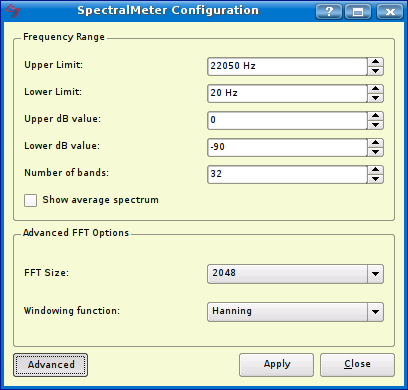
\includegraphics[width=0.5\textwidth]{../images/fft3.png}
	\caption{Una ventana de configuración, invocada con \sact{E}, permite configurar varios parámetros del analizador de espectros FFT.}
	\label{fig_fft3}
\end{figure}

\emph{Nota:} Para tamaños muy grandes de FFT, la velocidad de refresco visual del analizador de espectros se vuelve lenta. Esto no es causado necesariamente por sobrecarga de la CPU (aunque el uso de CPU aumenta con el tamaño de la FFT), sino que de hecho lleva cierto tiempo llenar los búferes con cantidades de datos tan grandes. El programa espera hasta que el búfer esté lleno antes de actualizar el trazado.

\section{Procesado externo}
Traverso permite procesar clips de audio usando programas externos como ``sox'' \cite{sox}, lo que aumenta todavía más las posibilidades de aplicar efectos. Esta característica es particularmente útil para acciones como cambiar la frecuencia de muestreo, anular la componente de corriente continua de la señal, invertir la fase, etc. En Linux, el programa ``sox'' debe estar instalado en el sistema. Está disponible en el repositorio de las principales distribuciones. En Windows y Mac OS X el instalador se ocupa de todas las dependencias.

\begin{figure}
	\centering
	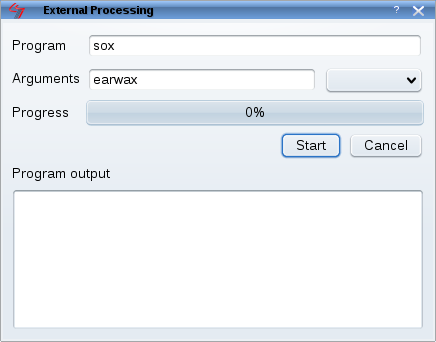
\includegraphics[width=0.5\textwidth]{../images/external00}
	\caption{Pulsando \sact{E} en un clip de audio, se abre la ventana de edición del clip. En ella, pulsando en ``Procesado externo'' se abre otra ventana que permite usar un programa externo para aplicar efectos.}
	\label{fig_external01}
\end{figure}

Como sabemos, el editor de propiedades del clip se abre pulsando \sact{E} sobre el clip (\FigB~\ref{fig_external01}). Pulsando  el botón ``Procesado externo'' de esa ventana, aparece la ventana de control del procesado externo (\FigB~\ref{fig_external01} dcha.). Deje el primer campo con ``sox'', y seleccione un efecto en el campo ``Argumentos''. Deje siempre el nombre del argumento en ese campo, y añada sus propios argumentos adicionales. Traverso usará esta primera entrada para etiquetar el archivo convertido. ¿No lo entiende bien? Vale, veamos un ejemplo. Supongamos que queremos invertir la fase del archivo myfile.wav. Lo importamos en Traverso, pulsamos \sact{E} en el clip, y en la ventana que sale, ``procesado externo''. Dejamos el campo ``sox'' como está, y seleccionamos el efecto ``vol'' del siguiente campo. Según el manual del programa sox, poniendo el volumen a $-1.0$ invertimos la fase, por tanto ponemos ``$-1.0$'' tras ``vol'' (sin las comillas). Pulsamos ``Start'' y esperamos hasta que el procesado termine. Traverso reemplazará automáticamente el clip con la versión procesada, que tendrá el nombre ``myfile-vol -1.0.wav''. Este fichero se guardará en el directorio ``audiosources'' que hay en el directorio del proyecto, sin importar dónde estuviese guardado el archivo original. Por tanto, éste no será sobreescrito nunca. Puede encontrarse más información sobre los efectos que proporciona el programa sox en sus ´´man pages'', a las que puede accederse poniendo``man:sox'' en la barra de direcciones de Konqueror, o ``man sox'' desde terminal.

